\documentclass[twocolumn]{article}

\usepackage[margin=0.68in,columnsep=0.22in]{geometry}
\usepackage[T1]{fontenc}
\usepackage{amsmath}
\usepackage{booktabs}
\usepackage{graphicx}
\usepackage[numbers,sort&compress]{natbib}

\graphicspath{{figures/}}
\setlength{\tabcolsep}{3pt}
\renewcommand{\arraystretch}{1.05}

\title{Supplementary Material:\\When MRI Slice Interpolators Disagree}
\author{Anonymous Authors}
\date{}

\begin{document}
\maketitle

\section{Reproducibility Scope}

All primary results use complete evaluation profiles: 115 IXI examinations, 24 fastMRI-brain examinations, and 22 held-out NingXia examinations pooled across eight cross-validation folds. Predictions are matched by case identifier and checked for equal volume shape before scoring. The factor-four protocol evaluates slice indices not divisible by four. No reconstruction model is trained as part of the committee analysis.

For target model $m$, the all-member committee contains linear and cubic interpolation plus every available neural output except $m$. The neural committee removes linear and cubic; the analytical committee retains only those two references. The main voxel score is the median absolute target-to-member difference. Examination scores average this map inside a mask derived from the target prediction at 1\% of its maximum absolute intensity.

\section{Bootstrap Intervals}

Table~\ref{tab:main-ci} reports 95\% intervals from 2,000 case-bootstrap replicates for the four primary endpoints. Resampling is paired within a target--dataset result. For nAURC and RRR, the complete ranking and its random and oracle references are recomputed in every replicate. All foreground pixel-correlation, case-Spearman, and RRR$_{50}$ intervals exclude zero, although the small-cohort intervals remain wide and should not be interpreted as evidence of a stable deployment threshold.

\begin{table*}[t]
  \centering
  \caption{Primary point estimates with case-bootstrap 95\% intervals. RRR$_{50}$ is expressed as a percentage.}
  \label{tab:main-ci}
  \resizebox{\textwidth}{!}{\begin{tabular}{llrrrr}
\toprule
Dataset & Target & $n$ & Pixel $r$ & Case $\rho$ & nAURC / RRR$_{50}$ \\
\midrule
IXI & ACSI & 115 & 0.435 [0.428,0.441] & 0.954 [0.923,0.972] & 0.035 [0.018,0.060] / 50.1 [46.1,54.8]\% \\
IXI & HAT & 115 & 0.511 [0.503,0.519] & 0.966 [0.940,0.980] & 0.024 [0.012,0.042] / 49.6 [45.4,53.9]\% \\
IXI & I$^3$Net & 115 & 0.351 [0.346,0.357] & 0.951 [0.922,0.969] & 0.044 [0.024,0.073] / 52.1 [45.9,55.9]\% \\
IXI & SwinIR & 115 & 0.519 [0.511,0.527] & 0.965 [0.939,0.980] & 0.025 [0.012,0.043] / 49.5 [45.1,53.6]\% \\
fastMRI & HAT & 24 & 0.325 [0.293,0.360] & 0.916 [0.761,0.962] & 0.067 [0.017,0.176] / 19.7 [11.7,26.1]\% \\
fastMRI & I$^3$Net & 24 & 0.289 [0.260,0.321] & 0.890 [0.721,0.962] & 0.092 [0.030,0.187] / 19.3 [10.8,25.8]\% \\
fastMRI & SwinIR & 24 & 0.359 [0.325,0.395] & 0.931 [0.780,0.978] & 0.061 [0.013,0.158] / 20.5 [12.6,26.9]\% \\
NingXia & HAT & 22 & 0.277 [0.256,0.296] & 0.929 [0.786,0.974] & 0.076 [0.016,0.239] / 22.2 [12.8,31.3]\% \\
NingXia & I$^3$Net & 22 & 0.355 [0.331,0.376] & 0.914 [0.774,0.968] & 0.063 [0.016,0.189] / 23.1 [12.6,32.7]\% \\
NingXia & SwinIR & 22 & 0.279 [0.256,0.300] & 0.936 [0.804,0.985] & 0.036 [0.007,0.120] / 21.4 [12.2,31.2]\% \\
\bottomrule
\end{tabular}
}
\end{table*}

\section{Committee Composition}

Figure~\ref{fig:composition} gives target-level nAURC rather than only the dataset averages reported in the main text. Mean all/neural/analytical nAURC is 0.032/0.033/0.059 on IXI, 0.073/0.017/0.118 on fastMRI, and 0.058/0.094/0.031 on NingXia. Thus, neural peers are strongest on fastMRI and analytical references on NingXia. This reversal is evidence against choosing one committee composition after observing test errors; the all-member committee is retained as the pre-specified main analysis.

\begin{figure*}[t]
  \centering
  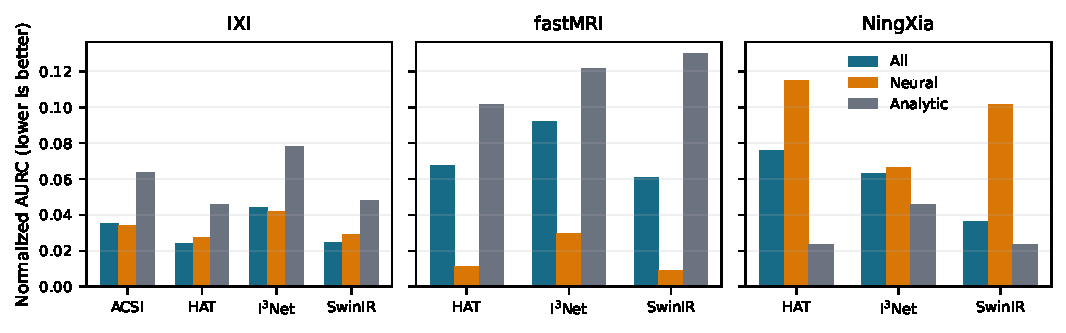
\includegraphics[width=0.96\textwidth]{figure3_committee_composition.pdf}
  \caption{Target-level committee-composition sensitivity. Lower normalized AURC indicates a ranking closer to the oracle. Differences across targets expose correlated errors and dependence on analytical references.}
  \label{fig:composition}
\end{figure*}

\section{Leave-One-Member-Out Analysis}

For each target and examination, we first average the target-to-member absolute difference inside the deployment-compatible foreground mask. We then remove one member and take the median of the remaining member scores. This score-level analysis is intentionally distinguished from the voxel-level main method: it tests whether examination ranking depends critically on one committee member without claiming an identical spatial map after removal. Complete results are provided in the machine-readable composition and leave-one-out report CSVs.

\section{Proxy Comparisons}

The all-member target-specific score is compared with neural-only disagreement, analytical-only disagreement, shared committee dispersion, and residuals to linear and cubic interpolation. Pixel-correlation differences use paired case bootstrap resampling. Ranking differences recompute nAURC after paired case resampling. Relative to shared dispersion, target-specific disagreement lowers nAURC by 0.011--0.025 for all four IXI targets with intervals excluding zero; differences on fastMRI include zero, and NingXia is mixed. Complete estimates and intervals are stored in \texttt{paired\_proxy\_bootstrap.csv}; retaining the machine-readable table avoids an unreadable multi-page matrix in the manuscript.

TTA variance is treated as an auxiliary source of sensitivity rather than a direct substitute for committee disagreement. It requires repeated inference and measures transformation response, whereas the proposed score measures inconsistency across reconstructors. Full-profile TTA, calibration-bin, failure-ranking, and reconstruction-context results are retained as machine-readable supplementary assets. They are not used to claim superiority for the corrected target-specific score because the earlier baseline-disagreement analysis used a shared committee map.

\section{Failure Detection and Interpretation}

Binary failures are defined retrospectively as the highest-MAE 10\% of examinations for each target model. This gives 12 positives on IXI and only three positives on each smaller cohort. AUROC, AUPRC, and top-$k$ recall are therefore supplementary endpoints. The risk--coverage curve remains primary because it uses continuous reconstruction error and directly represents review workload.

High disagreement can be correct when a target preserves structure smoothed by other methods. Low disagreement can be wrong when committee members share a bias. The qualitative selection in the main paper includes both a useful referral and a false-reassurance example to make this boundary visible.

\section{Artifact Traceability}

The analysis writes per-case scores, per-member scores, summary metrics, risk curves, and failure tables into profile-specific directories. Statistical reports consume only those CSV files. Paper tables and figures consume only the report and profile CSVs and write an \texttt{asset\_source\_manifest.csv}. A final consistency check verifies required artifacts, formatted main-table values, forbidden screening-profile claims, and unresolved LaTeX references.

\end{document}
